%
% positiv.tex
%
% (c) 2021 Prof Dr Andreas Müller, OST Ostschweizer Fachhochschule
%
\documentclass[tikz]{standalone}
\usepackage{times}
\usepackage{amsmath}
\usepackage{txfonts}
\usepackage[utf8]{inputenc}
\usepackage{graphics}
\usetikzlibrary{arrows,intersections,math}
\usepackage{ifthen}
\begin{document}

\newboolean{showgrid}
\setboolean{showgrid}{false}
\def\breite{7}
\def\hoehe{4}

\begin{tikzpicture}[>=latex,thick]

% Povray Bild
\node at (0,0) {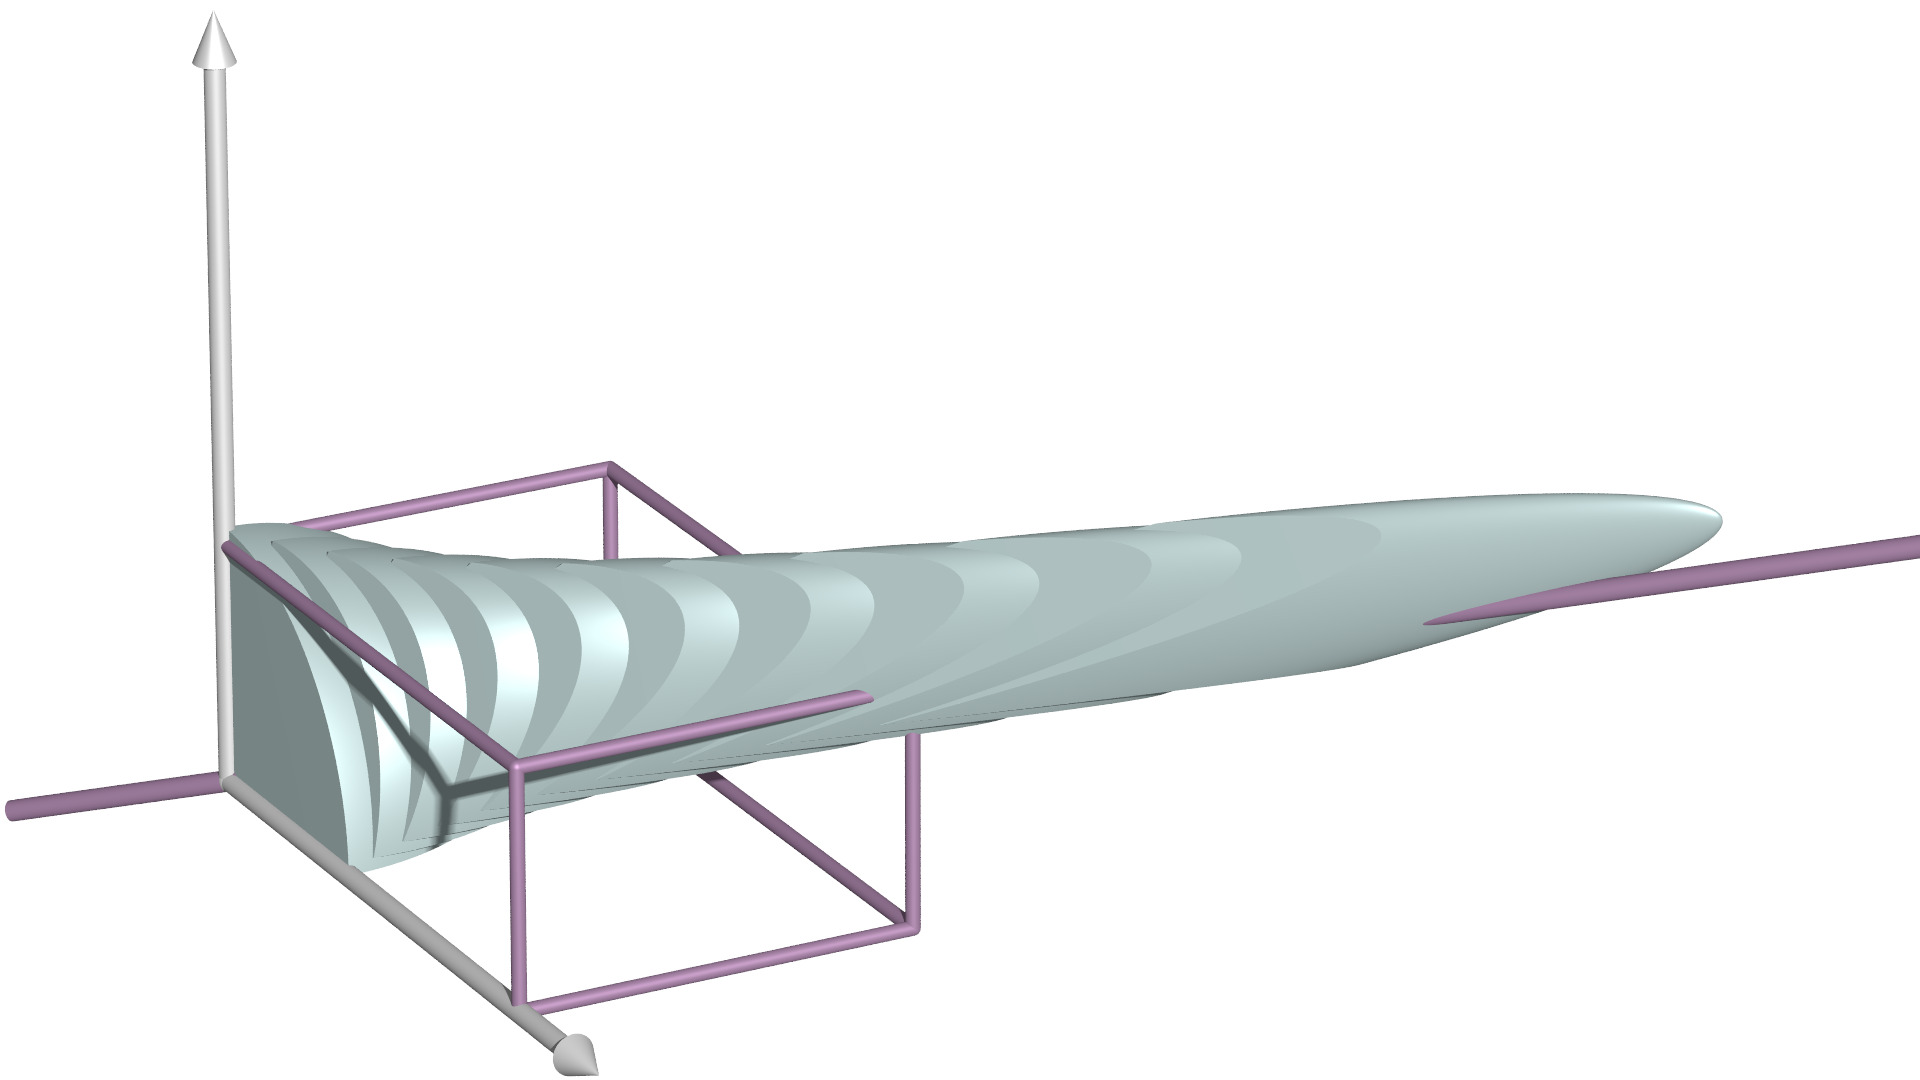
\includegraphics[width=14cm]{positiv.jpg}};

% Gitter
\ifthenelse{\boolean{showgrid}}{
\draw[step=0.1,line width=0.1pt] (-\breite,-\hoehe) grid (\breite, \hoehe);
\draw[step=0.5,line width=0.4pt] (-\breite,-\hoehe) grid (\breite, \hoehe);
\draw                            (-\breite,-\hoehe) grid (\breite, \hoehe);
\fill (0,0) circle[radius=0.05];
}{}

\node at (-2.6,-3.8) [right] {$x_1$};
\node at (-5.4,3.8) [right] {$x_3$};

\node[color=red] at (-4.5,-1.3) {$0$};
\node[color=red] at (-4.15,-1.25) {$1$};
\node[color=red] at (-3.75,-0.90) {$2$};
\node[color=red] at (-3.22,-0.80) {$3$};
\node[color=red] at (-2.6,-0.70) {$4$};
\node[color=red] at (-1.8,-0.60) {$5$};
\node[color=red] at (-0.9,-0.50) {$6$};
\node[color=red] at (0.2,-0.40) {$7$};
\node[color=red] at (1.6,-0.20) {$8$};
\node[color=red] at (4.0,0.10) {$9$};

\end{tikzpicture}

\end{document}

